\section{Proof of \Cref{main: upper}}
\label{sec: planar}

\newcommand{\gluepath}{{\mathsf{Glue}}}
\newcommand{\cutpath}{{\mathsf{Cut}}}

In this section we provide the proof of \Cref{main: upper}. We will use a similar algorithmic framework as \cite{chang2022near}, by first considering the case where all terminals lie on the boundary of one face and then generalizing the arguments to the $O(1)$-face case and eventually to the general case.

Let $G,G'$ be planar graphs with $T\subseteq V(G),V(G')$.
Let $\fset$ be the set of faces in the planar drawing of $G$ that contain all terminals, and we define $\fset'$ similarly for $G'$.
We say instances $(G,T),(G',T)$ are \emph{aligned}, iff there is a one-to-one correspondence between sets $\fset$ and $\fset'$, such that for each face $F\in \fset$, the set of terminals in $G$ lying on $F$ is exactly the set of terminals in $G'$ lying on $F'$, its corresponding face in $\fset'$, and the circular ordering in which these terminals appear on $F$ and $F'$ are also identical.
We say $(G,T)$ is a $|\fset|$-face instance. Throughout this section, all the cut sparsifiers that we will ever construct for the input instance or any subinstance generated from it are aligned.

\subsection{Preparation: removing separator terminals, and dual graphs}

We start with the following divide and conquer lemma, whose proof is deferred to \Cref{apd: Proof of lem: divide}.

\begin{lemma}
\label{lem: divide}
Let $(G,T)$ be a planar instance and let $\gset$ be a collection of subgraphs of $G$ such that the edge sets $\set{E(G') \mid G'\in \gset}$ partition $E(G)$. For each graph $G'\in \gset$, we denote by $T_{G'}$ the set that contains all vertices in $T\cap V(G')$ and all vertices of $G'$ that appear in some other graph in $\gset$.
If for each $(G',T_{G'})$ we are given a quality-$q$ aligned cut sparsifier $(H_{G'}, T_{G'})$, then we can efficiently obtain a quality-$q$ planar cut sparsifier $H'$ of $G$ with $|V(H')|\le \sum_{G'\in \gset}|V(H_{G'})|$.
\end{lemma}

We say a vertex $v\in V(G)$ is a \emph{separator} iff $G\setminus v$ is disconnected.
Denote its connected components by $G'_1,\ldots,G'_r$.
For each $1\le i\le r$, let $G_i$ be the subgraph of $G$ induced by $V[G'_i]\cup \set{v}$. We say graphs $G_1,\ldots,G_r$ are obtained by \emph{splitting $G$ at $v$}.
We use the following lemma from \cite{chang2022near}.

\begin{claim}[Claim 4.3 in \cite{chang2022near}]
\label{clm: separator}
Let $(G,T)$ be an instance.
Let $U$ be the set of separators in $T$. Let $\gset$ be the set of graphs obtained by splitting $G$ at all vertices in $U$ (that is, we first split $G$ at a vertex in $U$, and then repeatedly split each of the obtained graph at one of its separator terminal, until no resulting graph contains any separator terminal). Then
$\sum_{G'\in \gset}|T\cap V(G')|\le O(|T|)$.
\end{claim}

With \Cref{lem: divide}, we will assume that no terminal in $T$ is a separator in $G$, and so if we go around the boundary of a face in $\fset$, we will visit each terminal that lies on this face exactly once. This is since we can split $G$ at all its separator terminals, compute quality-$(1+\eps)$ cut sparsifiers for them separately, and then combine them in the way of \Cref{lem: divide}, paying only an $O(1)$ factor in the total size, as guaranteed by \Cref{clm: separator}.

\paragraph{Dual graphs.}
Cuts in planar graphs are cycles in their dual graphs. We will exploit this property in a similar way as \cite{krauthgamer2017refined} and transform the cut-preserving tasks to distance-preserving tasks. For technical reasons, in order to handle graphs with terminals, our definition of dual graphs are slightly different from the standard planar dual graphs.

Let $(G,T)$ be the input instance and let $\fset$ be the faces that contains all terminals.
Assume each face is a simple cycle. For each $F\in \fset$, add an auxiliary vertex $x_F$, and connect it to every terminal via a new edge, such that these edges are drawn in an internally disjoint way within face $F$, so that they separates face $F$ into subfaces, which we call special subfaces. Then we take the standard planar dual of the modified graph.
Here each special face correspond to a node, which we call \emph{dual terminals}. We then remove all edges in the dual graph connecting a pair of dual terminals. We denote the resulting graph by $G^*$, and denote by $T^*$ the set of dual terminals. See \Cref{fig: dual} for an illustration.
Note that when graph $G$ does not have the property that each face is a simple cycle, as long as we are guaranteed that no terminal is a separator, we can still define dual graphs similarly.
It is also easy to verify that the dual of the dual graph $G^*$ is the original graph $G$ itself. Sometimes we say that we \emph{reverse} $G^*$ to obtain $G$.
Finally, as both $G$ and $G^*$ are planar graphs, and each non-terminal vertex in $G^*$ corresponds to a face in $G$, the number of vertices in $G$ and $G^*$ are within $O(1)$ factor from each other.


\begin{observation}
	$(G,T)$ is a $f$-face instance iff $(G^*,T^*)$ is a $f$-face instance.
\end{observation}
We denote by $\fset^*$ the faces in $G^*$ that contain all dual terminals. It is easy to see that there exists a natural one-to-one correspondence between $\fset$ and $\fset^*$.

\begin{figure}[h]
	\centering
	\subfigure%[A metric $D$ on points $a,b,c$.]
	{\scalebox{0.1}{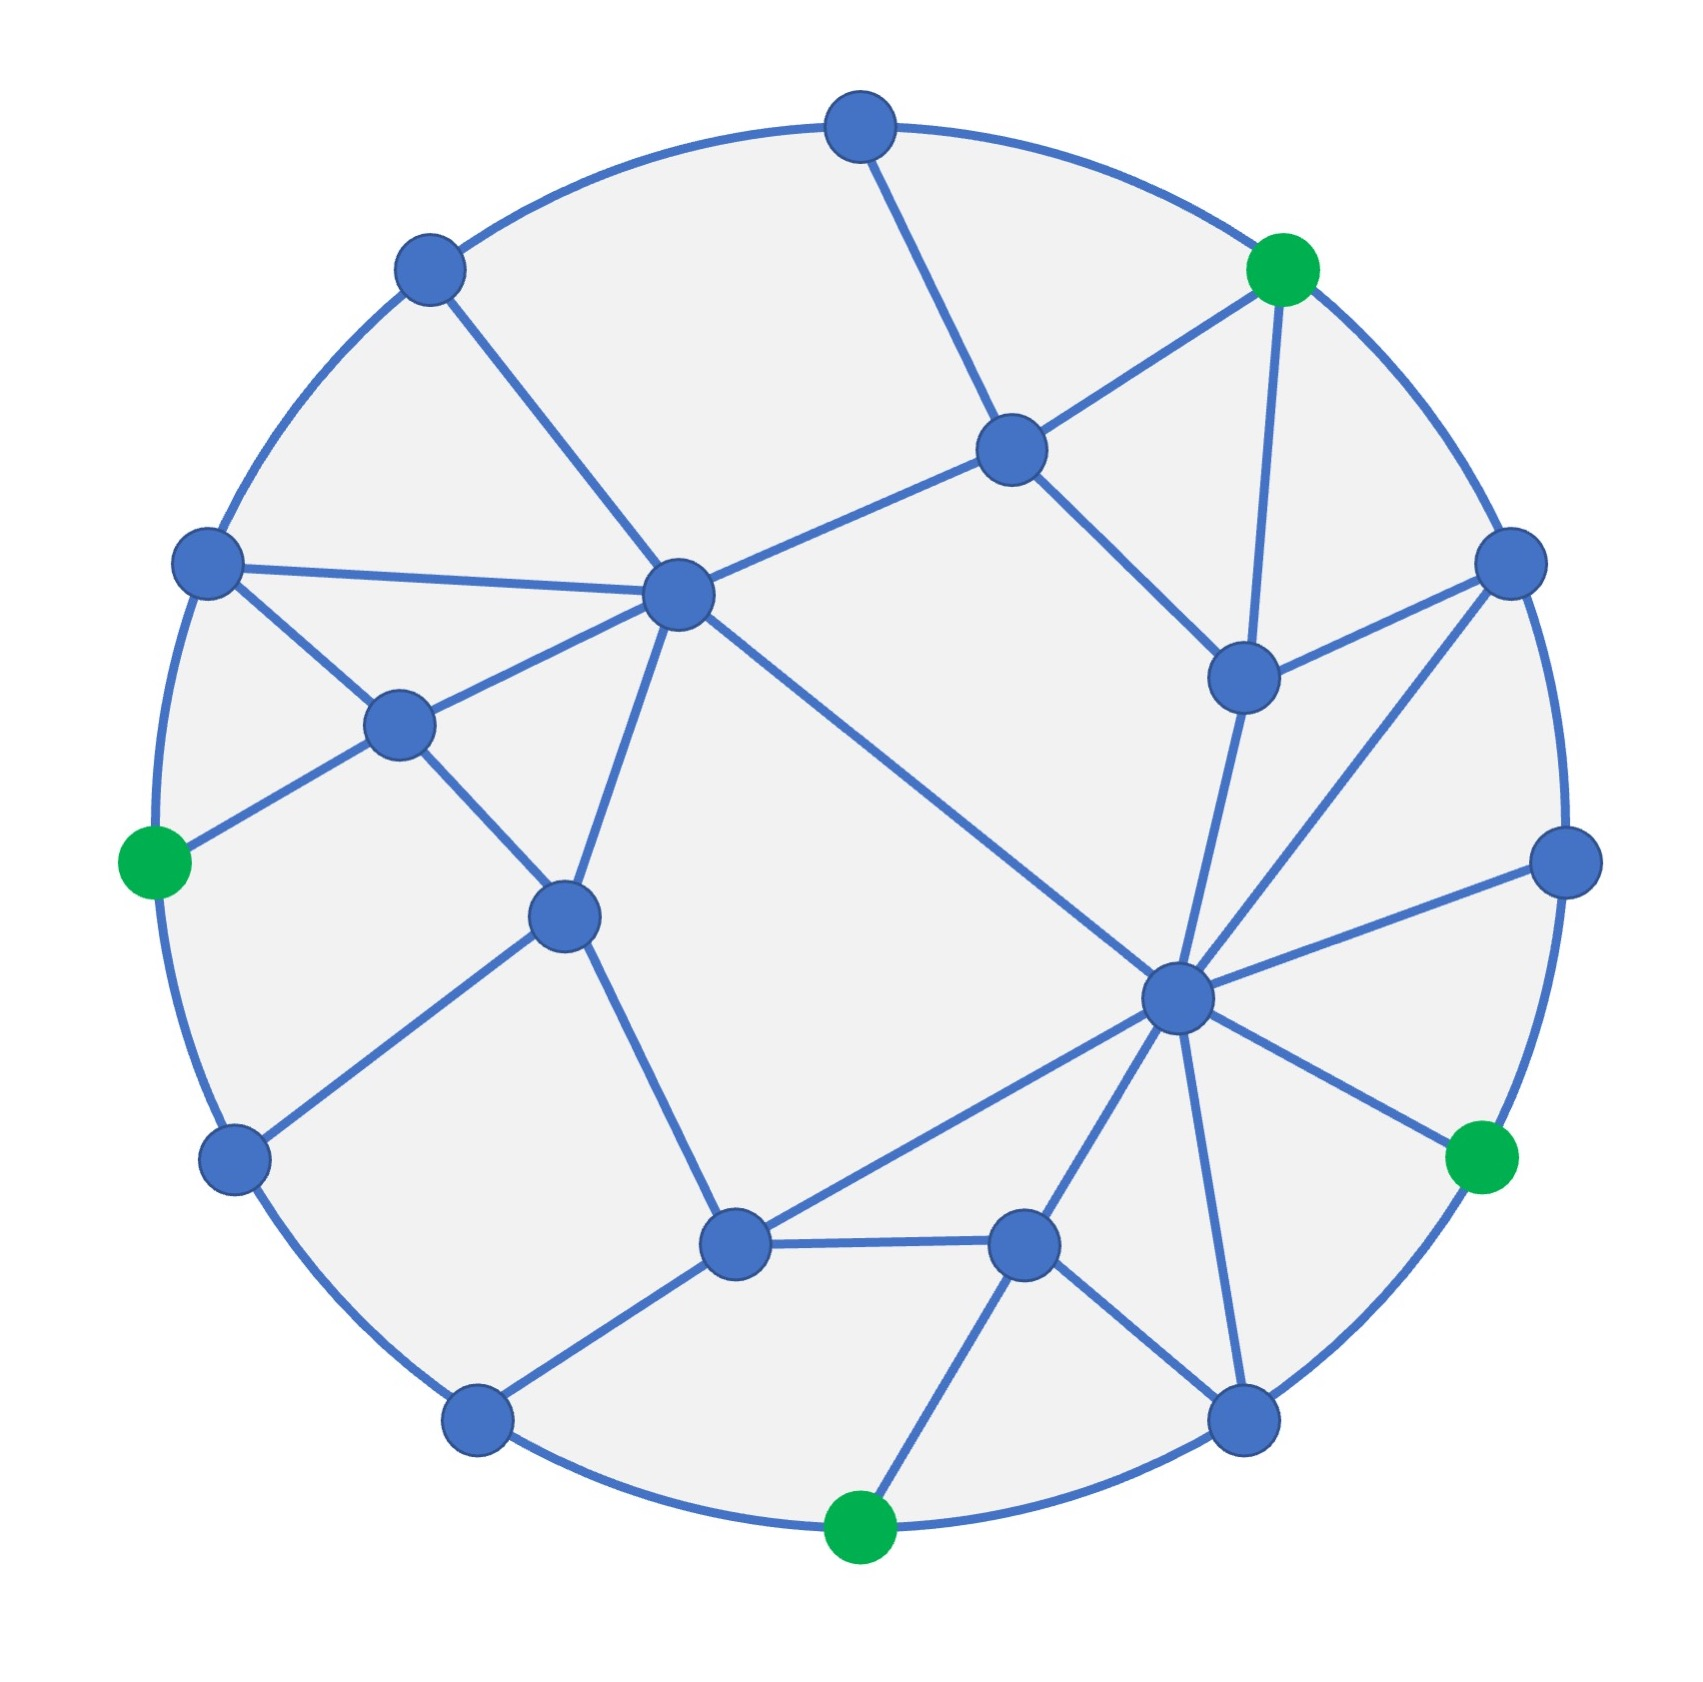
\includegraphics{fig/1face_1}}}
	\hspace{0.7cm}
	\subfigure%[The tight span $\TS(D)$.]
	{
		\scalebox{0.1}{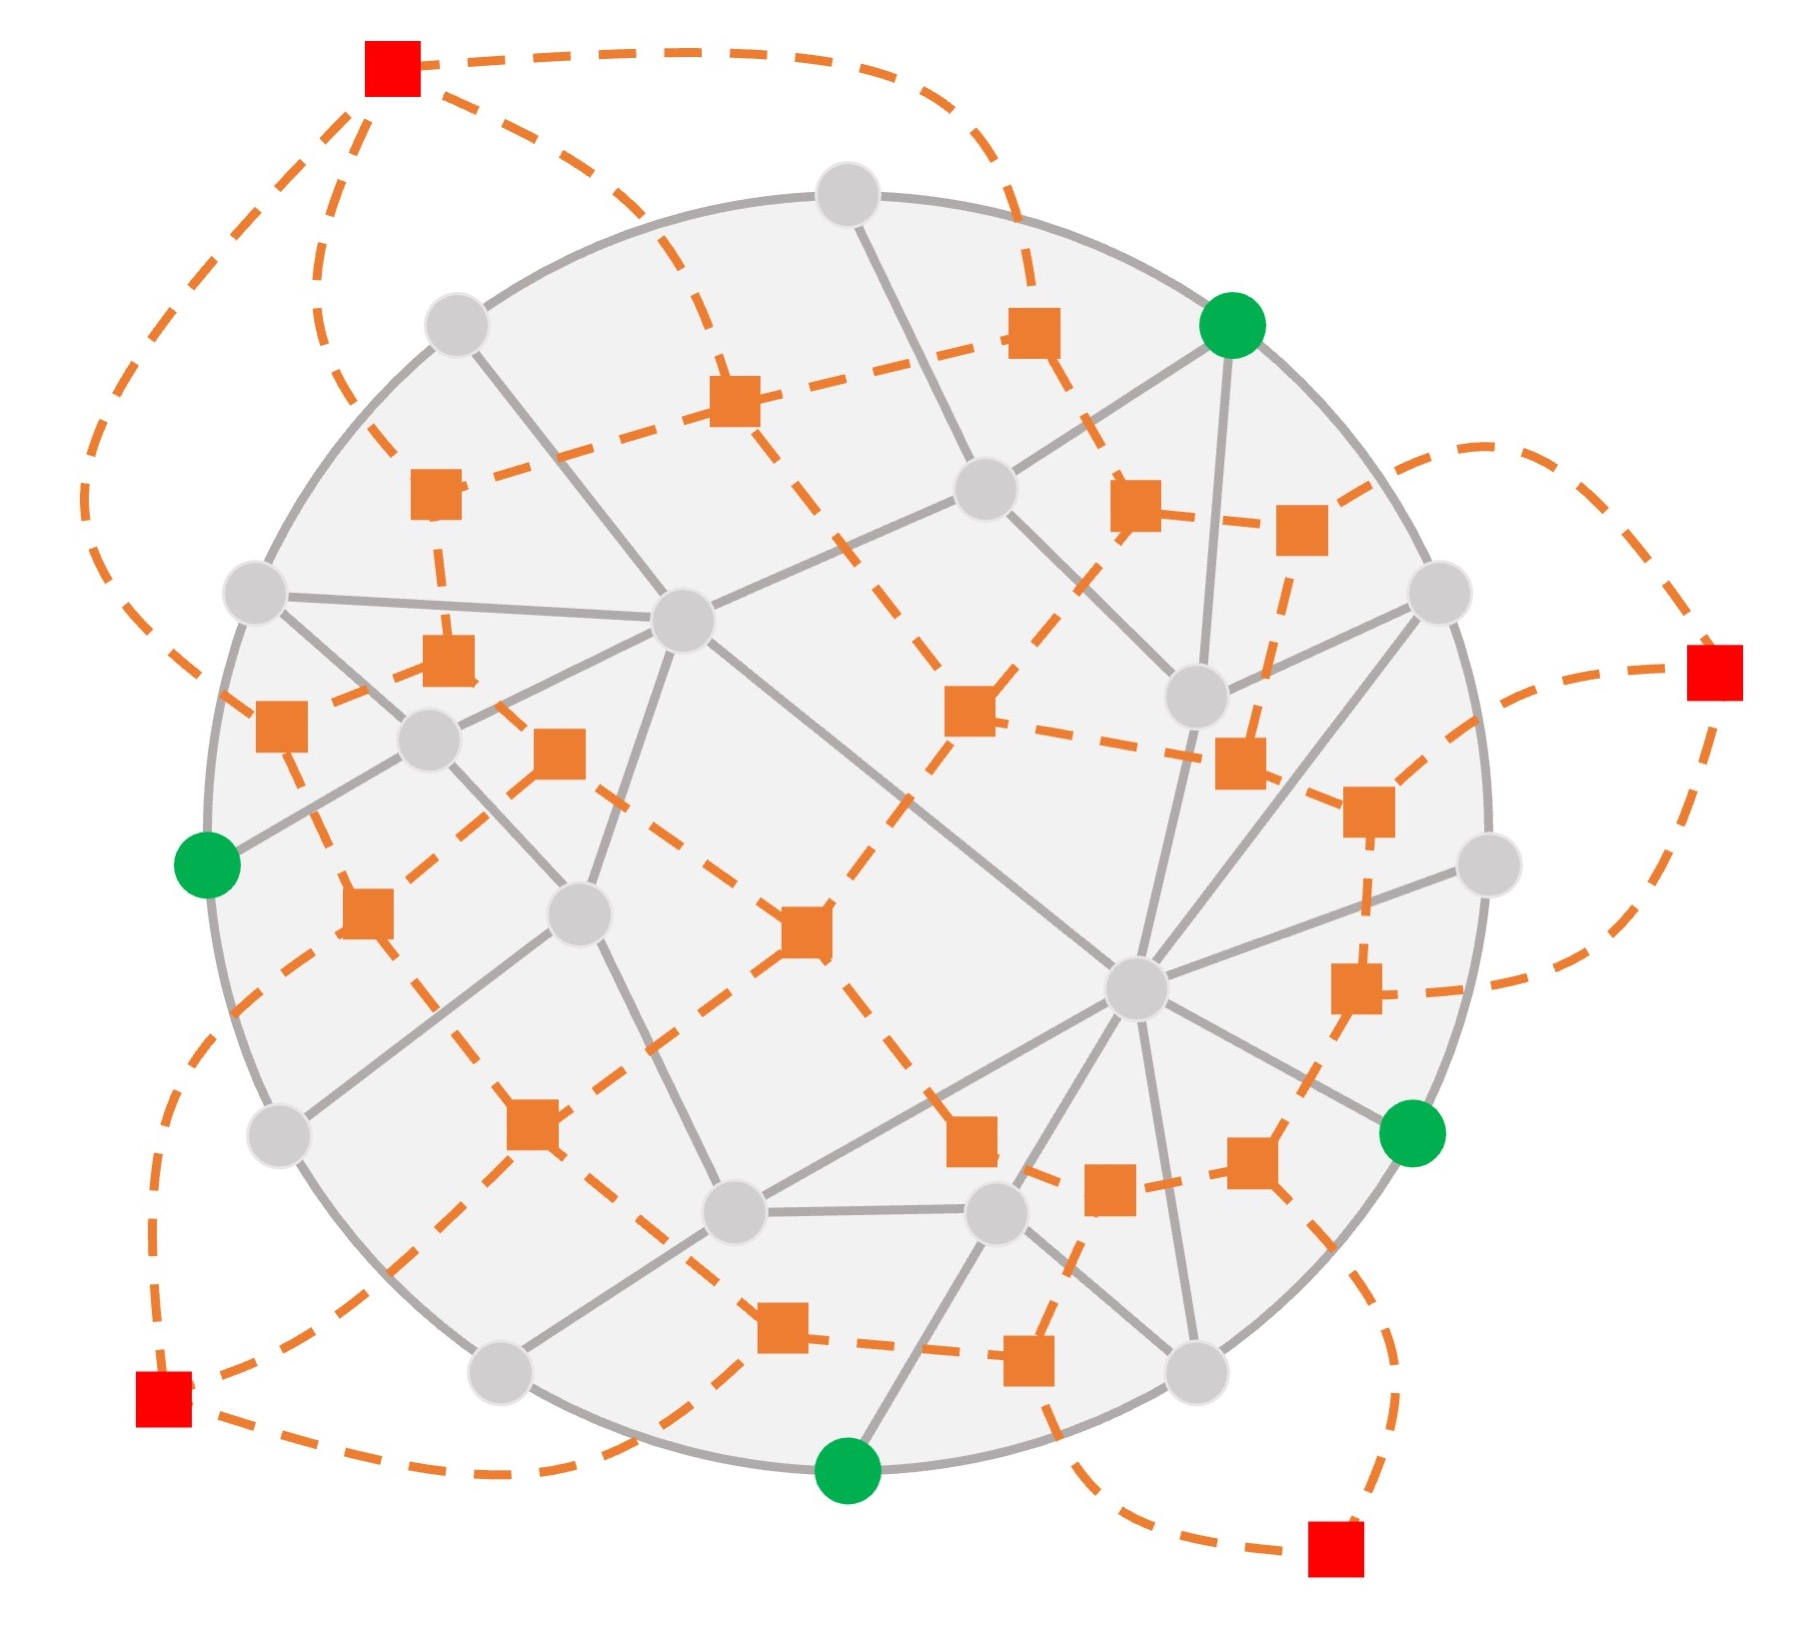
\includegraphics{fig/1face_2}}}
	\caption{An illustration of a one-face instance $(G,T)$ (left) and its dual $(G^*,T^*)$ defined in our way (right). The dual terminals in $T^*$ are marked in red. Taking the dual of (or reverse) $G^*$ we get $G$ back.\label{fig: dual}}
\end{figure}



\subsection{Warm-up: the one-face case}
\label{sec: 1-face}

In this subsection we prove \Cref{main: upper} for the special case where all terminals lie on the boundary of the outer face in the planar embedding of $G$.



\begin{lemma}
	\label{lem: mincut structure}
Let $(G,T)$ be a one-face instance. Then for any partition $(T_1,T_2)$ of the terminals into non-empty subsets, for any min-cut $\hat E$ in $G$ separating $T_1$ from $T_2$, the corresponding edge set $\hat E^*$ in the dual graph $G^*$ is the union of several edge-disjoint shortest paths connecting dual terminals.
\end{lemma}

\begin{proof}
	For every non-terminal vertex $v$ in $G$, we say that it is a \emph{$1$-node} iff in graph $G\setminus \hat E$, $v$ lies in the same connected component with some terminal in $T_1$, and we define \emph{$2$-nodes} similarly.
	
	\begin{observation}
		\label{obs: 1 vs 2}
		Every non-terminal $v$ in $G$ is either a $1$-node or a $2$-node, but not both, and every edge in $\hat E$ connects a $1$-node to a $2$-node.
	\end{observation}
	\begin{proof}
		As $\hat E$ is a cut separating terminals in $T_1$ from terminals in $T_2$, in $G\setminus \hat E$ every non-terminal cannot be both a $1$-node and a $2$-node, as otherwise some $T_1$ terminal lies in the same connected component with some $T_2$ terminal, a contradiction.
		
		Assume now that there is a vertex that is neither a $1$-node nor a $2$-node. Consider the connected component $C$ of $G\setminus\hat E$ that contains it, so $C$ contains no terminals. Consider any edge $e$ connecting an vertex in $C$ to a vertex $v'$ outside $C$, clearly $e$ belongs to $\hat E$.
		We claim that $\hat E\setminus e$ is also a cut separating $T_1$ from $T_2$, contradicting the minimality of $\hat E$.
%		
		In fact, if $v'$ is a $1$-node ($2$-node, resp.), then in $G\setminus (\hat E\setminus e)$ all vertices of $C$ are also $1$-nodes ($2$-nodes, resp.); and if $v'$ is neither a $1$-node nor a $2$-node, then in $G\setminus (\hat E\setminus e)$ all vertices of $C$ are neither $1$-nodes nor $2$-nodes. In either case, $T_1$ are still separated from $T_2$ in $G\setminus (\hat E\setminus e)$.
		
		It is now easy to see that every edge in $\hat E$ connects a $1$-node to a $2$-node, since otherwise we can remove such an edge from $\hat E$, still separating $T_1$ from $T_2$, contradicting the minimality of $\hat E$.
	\end{proof}


	Denote $T=\set{t_1,\ldots,t_k}$, where the terminals are indexed according to the order that they appear on the boundary of the outer face. An \emph{interval} is a subsequence $t_i,t_{i+1}\ldots,t_j$, such that all terminals $t_i,t_{i+1}\ldots,t_j$ lies in the same connected component in $G\setminus \hat E$ that does not contain $t_{i-1}, t_{j+1}$.
	We say that an interval is a $1$-interval ($2$-interval, resp.) if all its terminals lie in $T_1$ ($T_2$, resp.).
	
	\begin{observation}
		\label{obs: interval}
		There is an interval $T'$, such that in $G\setminus \hat E$, $T'$ is separated from $T\setminus T'$.
	\end{observation}
	\begin{proof}
		We find such an interval as follows. Consider any interval $T'$. If it is separated from $T\setminus T'$ in $G\setminus \hat E$, then we are done. If not, then it is connected to some other interval $T''$ in $G\setminus \hat E$. They separate the boundary of the outer face into two segments both containing some terminals, but the terminals in one segment are not connected to the terminals in the other segment. We then recurse on one of these segments, start with any interval. Eventually we will find a desired interval.
	\end{proof}
	
	Consider an interval $T'$ and let $C$ be the connected component in $G\setminus \hat E$ that contains $T'$. Assume without loss of generality that $T'\subseteq T_1$. Let $\delta(C)$ be the edges in $G$ with exactly one endpoint in $C$, so clearly $\delta(C)\subseteq \hat E$. 
	
	\begin{claim}
		\label{clm: interval cut}
		$\delta(C)$ is the min-cut in $G$ separating $T'$ from $T\setminus T'$.
	\end{claim}
	\begin{proof}
		Let $E'$ be the mincut in $G$ separating $T'$ from $T\setminus T'$. We show that $(\hat E\setminus \delta(C))\cup E'$ is a cut in $G$ separating $T_1$ from $T_2$. From the minimality of $\hat E$, this means that $w((\hat E\setminus \delta(C))\cup E')\ge w(\hat E)$, implying that $w(\delta(C))\le w(E')$, or equivalently, $\delta(C)$ is the min-cut in $G$ separating $T'$ from $T\setminus T'$.
		%
		In fact, from \Cref{obs: 1 vs 2}, all outside-of-$C$ endpoints of edges in $\delta(C)$ are $2$-nodes.
		Therefore, it is easy to verify that $\hat E\setminus \delta(C)$ is a cut in $G$ separating $T_1\setminus T'$ to $T_2\cup T'$. As $E'$ is a cut separating $T'$ from $T_2$, we conclude that $\hat E\setminus \delta(C))\cup E'$ separates $T_1$ from $T_2$.
	\end{proof}
	
	
	\Cref{clm: interval cut} implies that, in the dual graph $G^*$, the dual edges of edges in $\delta(C)$ form a shortest path connecting a pair of terminals in $T^*$.
	In other words, we have managed to extract part of the cut $\hat E$ that is a shortest path in $G^*$. We now recursively extract other parts using the following claim from the rest of $\hat E$.
	
	\begin{claim}
		\label{clm: recursive}
		$\hat E\setminus \delta(C)$ is a min-cut in $G$ separating $T_1\setminus T'$ from $T_2$.
	\end{claim}
	\begin{proof}
		On one hand, we have shown in the proof of \Cref{clm: interval cut} that $\hat E\setminus \delta(C)$ is a cut in $G$ separating $T_1\setminus T'$ to $T_2\cup T'$, so $\hat E\setminus \delta(C)$ does separate $T_1\setminus T'$ from $T_2$.
		%
		On the other hand, if we let $E'$ be a min-cut in $G$ separating $T_1\setminus T'$ from $T_2$, then via similar analysis as in proof of \Cref{clm: interval cut}, we can show that $\delta(C)\cup E'$ is a cut in $G$ separating $T_1$ from $T_2$, implying that $w(\hat E)\le w(\delta(C)\cup E')$ and so $w(\hat E\setminus \delta(C))\le w(E')$.
	\end{proof}
	According to \Cref{clm: recursive}, we are able to repeatedly extract subsets of edges in $\hat E$ that correspond to shortest paths in $G^*$, using \Cref{obs: interval} and \Cref{clm: interval cut}, until $\hat E$ becomes empty. This completes the proof of \Cref{lem: mincut structure}. 
\end{proof}


We are now ready to prove \Cref{main: upper} for one-face instances using \Cref{main: upper}.
We first construct the dual graph $G^*$, and use the result in \cite{chang2022near} to construct a quality-$(1+\eps)$ planar distance emulator $\hat G^*$ with size $O(k\cdot \poly(\log k/\eps))$, and then reverse it to get $\hat G$. 
From our definition of dual graphs and their reverse, $\hat G$ contains all terminals and $|V(\hat G)|=O(k\cdot \poly(\log k/\eps))$. It remains to show that $(\hat G,T)$ is a quality-$(1+\eps)$ cut sparsifier for $(G,T)$. 

Let $(T_1,T_2)$ be a partition of $T$.
On the one hand, the min-cut in $G$ separating $T_1$ from $T_2$ consists of several edge-disjoint dual terminal shortest paths in $G^*$, and as $\hat G^*$ is a $(1+\eps)$ aligned distance emulator for $G^*$, we can find, for each such dual terminal shortest path in $G^*$, a shortest path in $\hat G^*$ connecting its corresponding dual terminals, with at most $(1+\eps)$ times the length. By taking the union of the edges in all these paths in $\hat G^*$ (note however that these paths are not necessarily edge-disjoint in $\hat G^*$), we obtain an edge set in $\hat G$ separating $T_1$ from $T_2$ whose value is at most $(1+\eps)$ times the value of $\mc_G(T_1,T_2)$. 
On the other hand, we apply the same analysis, starting with a min-cut in $\hat G$ separating $T_1$ from $T_2$. As $G^*$ is also a $(1+\eps)$ aligned distance emulator for $\hat G^*$, we can derive similarly that $\mc_{\hat G}(T_1,T_2)\le (1+\eps)\cdot \mc_G(T_1,T_2)$.



\subsection{The $O(1)$-face case}

In this subsection we prove the following lemma.

\begin{lemma}
	\label{lem: O(1) face}
	There exists a universal constant $c>0$, such that for any real number $0<\eps<1$, every $f$-face instance $(H,U)$ has an aligned $f$-face instance $(H',U)$ as its quality-$(1+\eps)$ cut sparsifier, with $|V(H')|\le |U|\cdot (cf\log |U|/\eps)^{cf^2}$.
\end{lemma}

Terminal-separating min-cuts in $G$ dual-terminal shortest paths in our graph $G^*$. Therefore, from now on we focus on preserving dual-terminal shortest paths in $G^*$. Recall that $\fset^*$ is the collection of faces in $G^*$ that contains all dual terminals. The following notion is central in our algorithm.


\paragraph{Pattern-shortest paths, pattern distances, and pattern emulators.}
For a pair $t,t'$ of dual terminals in graph $G^*$, there are more than one way for them to be connected by a path, depending on how the path goes around other faces in $\fset^*$, called \emph{patterns},  A rigorous way of defining patterns was given in \cite{krauthgamer2017refined}, which we describe below.

Fix a point $\nu^*$ in the plane.
Let $\gamma$ be a closed curve (not necessarily simple). A vertex $v\notin \gamma$ is said to be \emph{inside} $\gamma$ iff any simple curve connecting $\nu^*$ to $v$ crosses $\gamma$ an odd number of times, otherwise it is said to be \emph{outside} $\gamma$.
%
For a pair $t,t'$ of dual terminals in $G^*$, we denote by $\Pi_{t,t'}$ the shortest path connecting them in $G^*$.
For every face $F\in \fset^*$, we place a point $z_F$ inside its interior. Consider now a path $P$ in $G^*$ connecting $t,t'$. Note that the union of $P$ and $\Pi_{t,t'}$ is a closed curve. Now the \emph{pattern} of $P$ is defined to be a $|\fset^*|$-dimensional vector $\pat(P)=(\phi_F)_{F\in \fset^*}$, where $\phi_F=1$ iff $z_F$ is inside the closed curve formed by the union of $P$ and $\Pi_{t,t'}$ and $\phi_F=-1$ iff $z_F$ is outside.

\begin{observation}
\label{obs: pattern}
Between every pair of terminals there are $2^{f}$ different patterns.
\end{observation}
\begin{proof}
As a pattern is a $|\fset^*|=|\fset|=f$-dimensional $+/-$ vector. There are $2^f$ possibilities.
\end{proof}

Let $P,P'$ be simple paths with same endpoints, the above definition of pattern implies that paths $P,P'$ \emph{have the same pattern} iff all points $\set{z_F}_{F\in \fset^*}$ lie outside the closed curve $P\cup P'$.
We will also consider paths $P,P'$ with one common endpoint $t$. Let $R$ be a path such that the other-endpoints of $P$ and $P'$ both lie on $R$. In this case we say that paths $P,P'$ have the \emph{same pattern with respect to $R$}, iff all points $\set{z_F}_{F\in \fset^*}$ lie ourside the closed curve formed by the union of $P$, $P'$, and the subpath of $R$ between the other-endpoint of $P$ and the other-endpoint of $P'$.


\iffalse
\begin{observation}
Let $F,F'$ be distinct faces and let $P$ be a path connecting a vertex on face $F$ to a vertex on face $F'$. Let $t,t'$ be terminals such that $\Pi_{t,t'}$ is vertex-disjoint from $P$.
Let $Q$ be any other $t$-$t'$ path with pattern where $\phi_F\ne \phi_{F'}$. Then $Q$ must cross $P$.
\end{observation}
\fi


For a pattern $\pat$, the $t$-$t'$ \emph{$\pat$-shortest path} is defined to be the shortest path among all $t$-$t'$ paths with pattern $\pat$. Its length is defined to be the \emph{$\pat$-distance} between $t,t'$, which we denote by $\dist^{\Phi}(t_1,t_2)$.
Let $(G,T), (H,T)$ be aligned instances. We say that $(H,T)$ is a \emph{quality-$q$ pattern emulator} of $(G,T)$, iff for every pair $t_1,t_2$ of terminals and every pattern $\pat$, the $\pat$-distance between $t_1,t_2$ in $G$ is within factor $q$ from the $\pat$-distance between $t_1,t_2$ in $H$.
We use the following result from \cite{krauthgamer2017refined}.

\begin{theorem}[Adaptation of Theorem 4.6 in \cite{krauthgamer2017refined}]
\label{thm: pattern for cut}
Let $(G,T),(H,T)$ be aligned instances. If the dual instance $(H^*,T^*)$ is a quality-$q$ pattern emulator of the dual instance $(G^*,T^*)$, then $(H,T)$ is a quality-$q$ cut sparsifier of $(G,T)$.
\end{theorem}




\subsection{Constructing pattern emulators}

We will now prove the following lemma, which, combined with \Cref{thm: pattern for cut}, implies \Cref{lem: O(1) face}.

\begin{lemma}
\label{lem: O(1) face emulator}
There exists a universal constant $c>0$, such that for any $0<\eps<1$, every $f$-face instance $(G,T)$ admits a quality-$(1+\eps)$ pattern emulator $(H,T)$ with $|V(H)|\le |T|\cdot (cf\log |T|/\eps)^{cf^2}$.
\end{lemma}

We prove \Cref{lem: O(1) face emulator} by induction on $f$. The base case where $f=1$ has been proved in \Cref{sec: 1-face}.
Assume that we are given a $f$-face instance $(G,T)$.
We will convert it into an $(f-1)$-face instance and apply the inductive hypothesis.
Throughout this subsection, we use the parameters $\eps'=\eps/2f^2$ and $\eps''=(1-1/f^2)\cdot \eps$.

We first pick a pair $t,t'$ of terminals that lie on distinct faces, denoted by $\alpha,\alpha'$, respectively, and compute the shortest path $\Pi_{t,t'}$ in $G$ connecting $t$ to $t'$, such that $\Pi_{t,t'}$ does not contain any terminal as inner vertices. Denote $\Pi=\Pi_{t,t'}$. Then we compute a set of vertices on $\Pi$ that we call \emph{portals}. 

\paragraph{Portals on $\Pi$.}
We use the notion of $\eps$-covers defined in \cite{klein1998fully,thorup2004compact}.
Let $R$ be a shortest path and let $v$ be a vertex that does not lie in $R$. An \emph{$\eps$-cover} of $v$ in $R$ is a set $C(v,R)$ of vertices, such that for any vertex $x\in R$, there exists some $y\in C(v,R)$, such that 
$\dist(v,x)\le \dist(v,y)+\dist(y,x)\le (1+\eps)\cdot\dist(v,x).$
It has been shown \cite{klein1998fully,thorup2004compact} that for every $\eps>0$, shortest path $R$ and vertex $v\notin R$, there exists an $\eps$-cover of $v$ in $R$ of size $O(1/\eps)$.
%
As we want to construct pattern emulators, we will need to modify the definition of $\eps$-covers into a ``pattern version'' accordingly, as follows.

Let $G$ be an $f$-face instance, $R$ be a shortest path in $G$ that does not intersect any face internally, and $v$ be a vertex that does not lie in $R$. 
Let $Q$ be a path connecting $v$ to some vertex in $R$, and let $\Phi$ be its pattern. A \emph{$\Phi$-respecting $\eps$-cover} of $v$ in $R$ is a set $C(v,R,\Phi)$ of vertices, such that for any vertex $x\in R$, there exists some $y\in C(v,R,\Phi)$, such that the shortest $v$-$y$ path with the same pattern as $\Phi$, concatenated with the $y$-$x$ subpath of $R$, is within factor $(1+\eps)$ in length with the shortest $v$-$x$ path with the same pattern as $\Phi$. In other words (slightly abusing the notations),
$$\dist^\Phi(v,x)\le \dist^\Phi(v,y)+\dist(y,x)\le (1+\eps)\cdot\dist^\Phi(v,x).$$
We use the following lemma, whose proof is similar to the previous result of $\eps$-cover and is deferred to \Cref{apd: Proof of lem: pattern cover}.

\begin{lemma}
\label{lem: pattern cover}
For any planar instance $G$, shortest path $R$ in $G$, vertex $v\notin R$, and pattern $\Phi$, there exists a $\Phi$-respecting $\eps$-cover of $v$ in $R$ of size $O(1/\eps)$.
\end{lemma}


We now define a set $Y$ of vertices on $\Pi$ as follows. For each terminal $t$ and for each pattern $\Phi$, let $Y_{t,\Phi}$ be the pattern-respecting $\eps'$-cover of $v$ in $R$ of size $O(1/\eps')$ given by \Cref{lem: pattern cover}. We then let set $Y=\bigcup_{t,\Phi}Y_{t,\Phi}$.
From \Cref{obs: pattern} and \Cref{lem: pattern cover}, 
$|Y|\le O(2^f\cdot |T|/\eps')$.





We then slice the graph $G$ open along the path $\Pi$ connecting faces $\alpha,\alpha'$.
Specifically, we duplicate path $\Pi$ into two copies $\Pi_1,\Pi_2$ and place them closely at two sides (which we call $1$-side and $2$-side, respectively) of its original image, such that the thin strip between them connect faces $\alpha,\alpha'$ into a single face $\beta$.
All vertices $x$ on $P$ into their copies $x_1,x_2$ ($x_1$ lies on $\Pi_1$ and $x_2$ lies on $\Pi_2$), including the terminals $t,t'$ that now have copies $t_1,t_2$ and $t'_1,t'_2$. All weights on edges remain the same. 
It is easy to verify that the obtained graph, which we denote by $G'$, is a $(f-1)$-face instance.
Let $T'$ be the set that contains all copies of terminals and portals in $Y$.
We then construct a quality-$(1+\eps'')$ pattern emulator $H'$ of $G'$ with respect to $T'$, and then glue, for each portal $y\in Y$, its copies $y_1,y_2$ back to their original vertex $y$. The resulting graph is denoted by $H$ and is returned as the pattern emulator for $G$.
For a complete description of the cut and glue operations, please refer to Appendix B of \cite{chang2022near}.
See \Cref{fig: splitting h-hole after} for an illustration.

\begin{figure}[h!]
	\centering
	\subfigure[Graph $G$: faces $\alpha, \alpha'$ (shaded gray), path $\Pi$ (blue), and portals (purple). ]{\scalebox{0.5}{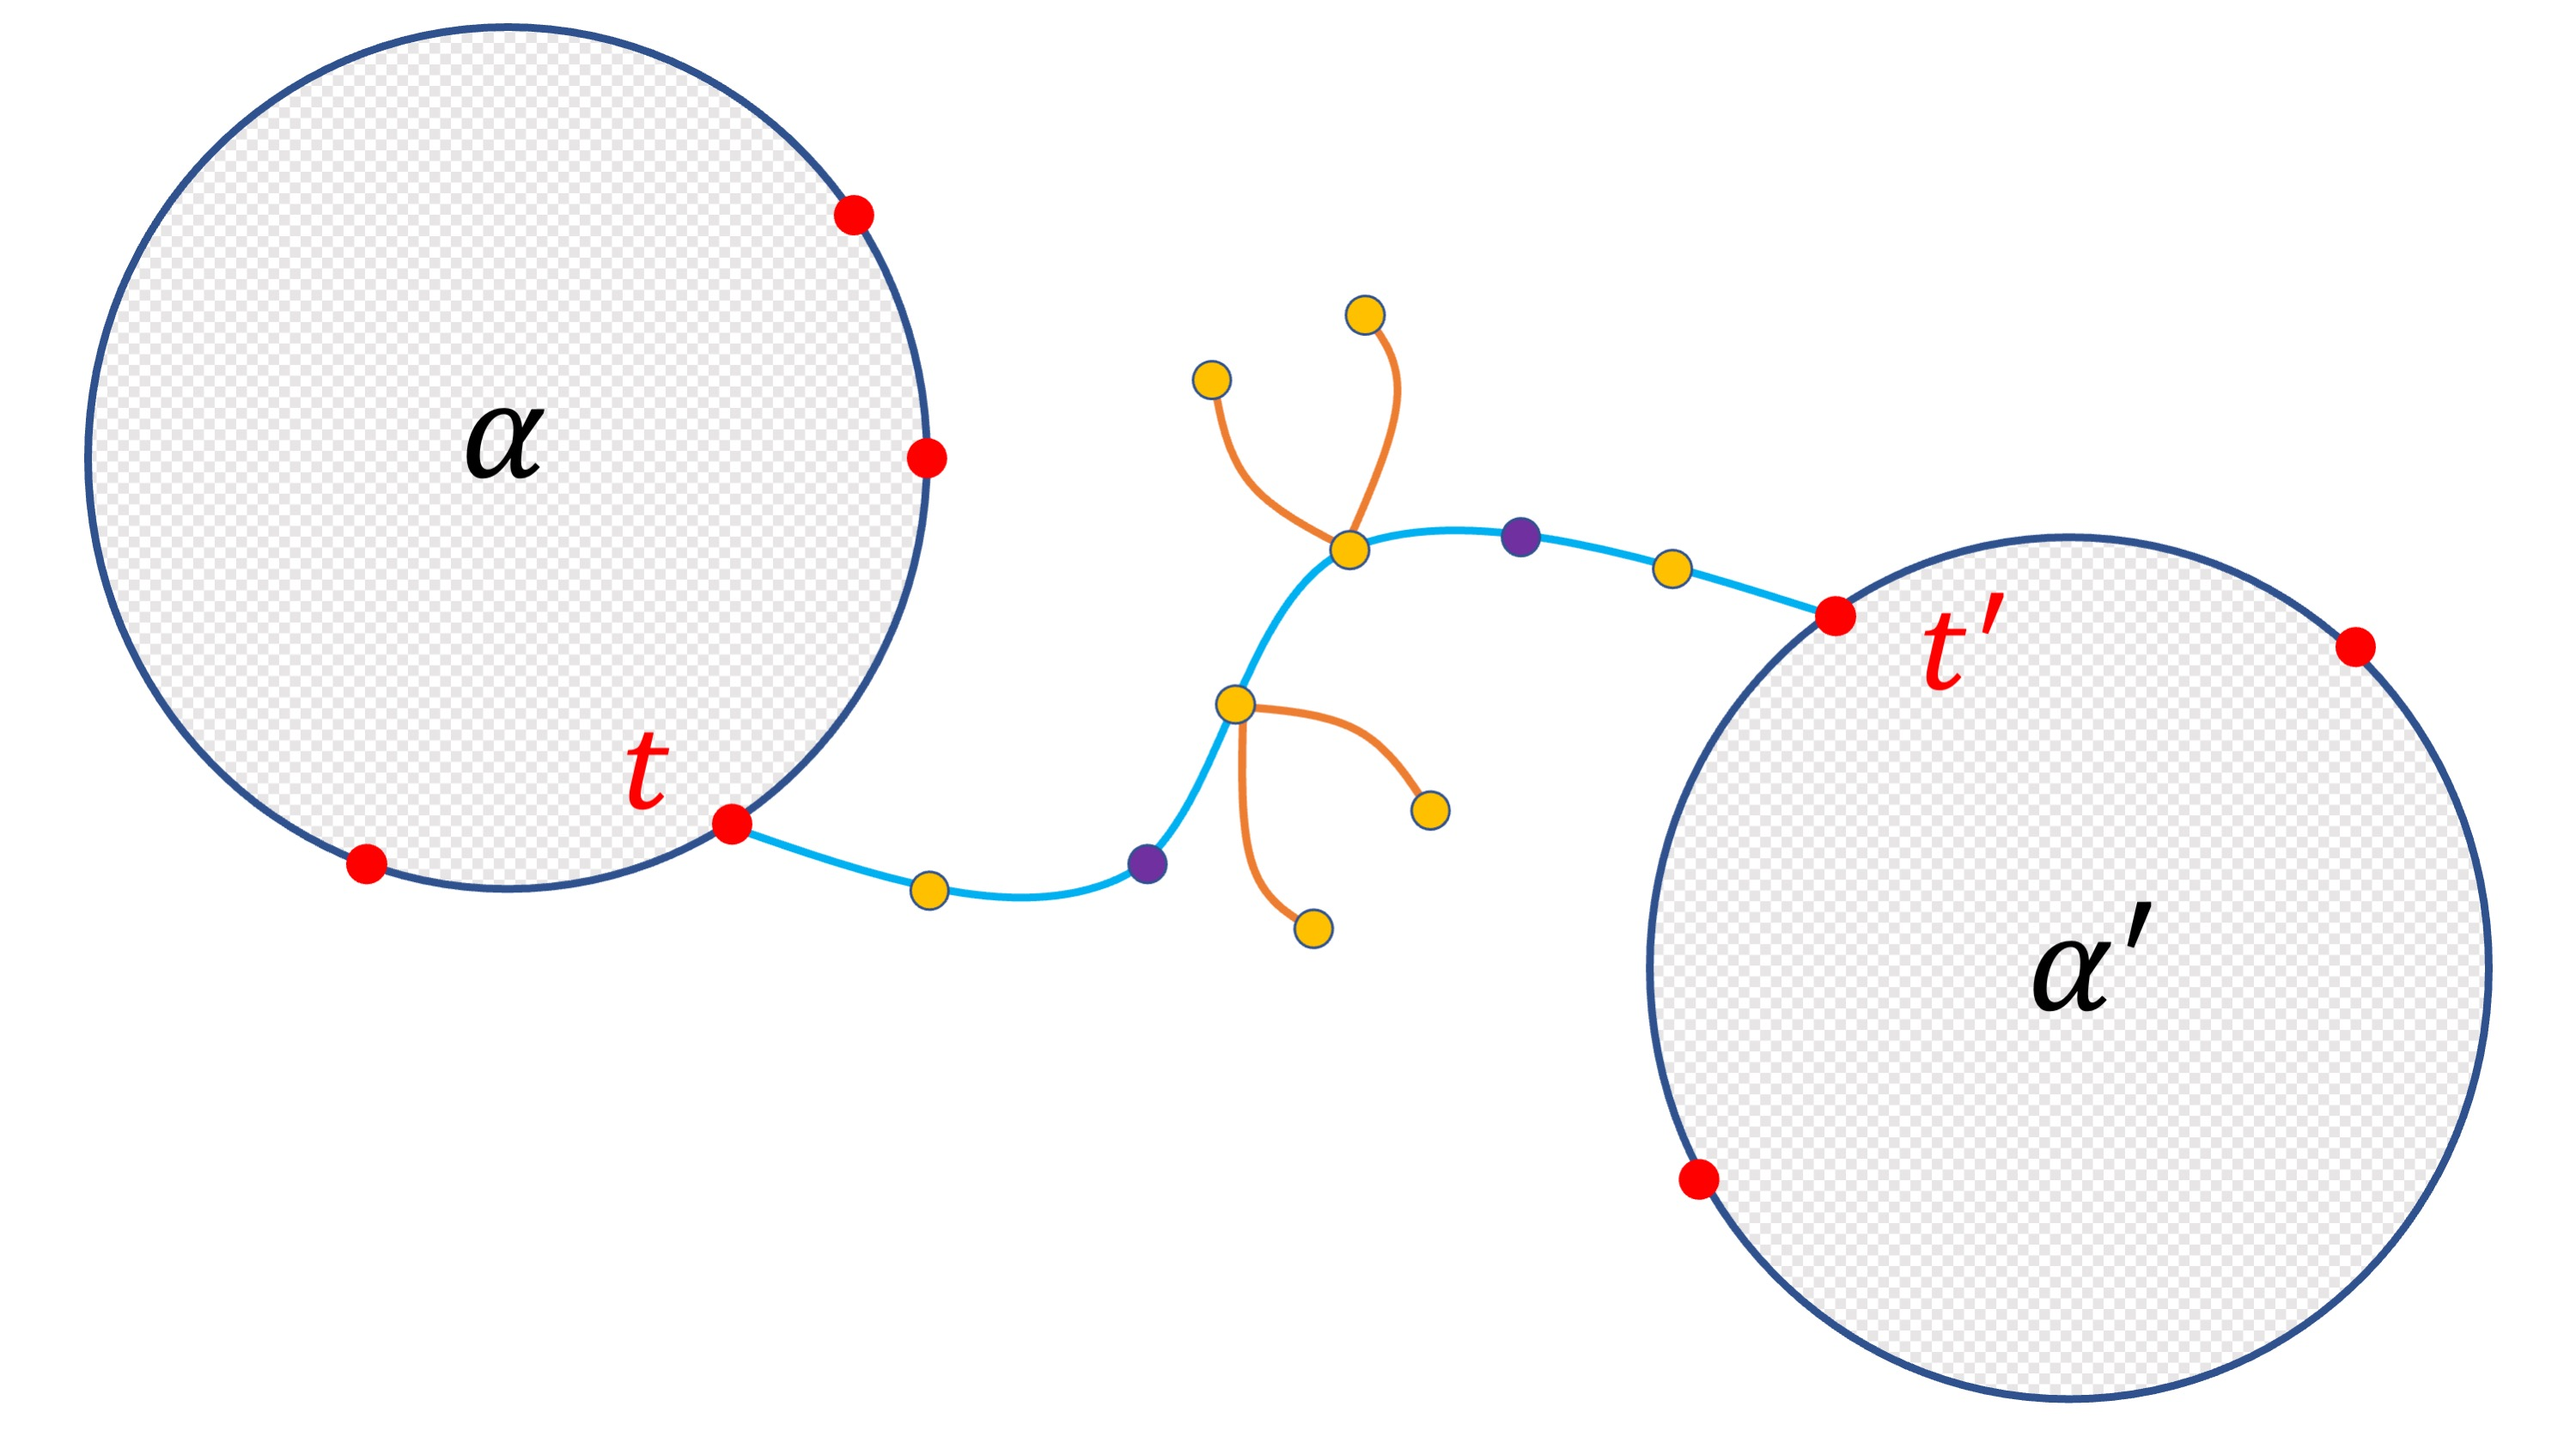
\includegraphics[scale=0.15]{fig/manyhole_1.jpg}\label{fig: splitting h-hole before}}}
	\hspace{0.2cm}
	\subfigure[Graph $G'$: the new hole $\beta$ (shaded gray), and paths $\Pi_1,\Pi_2$ (blue).]{\scalebox{0.5}{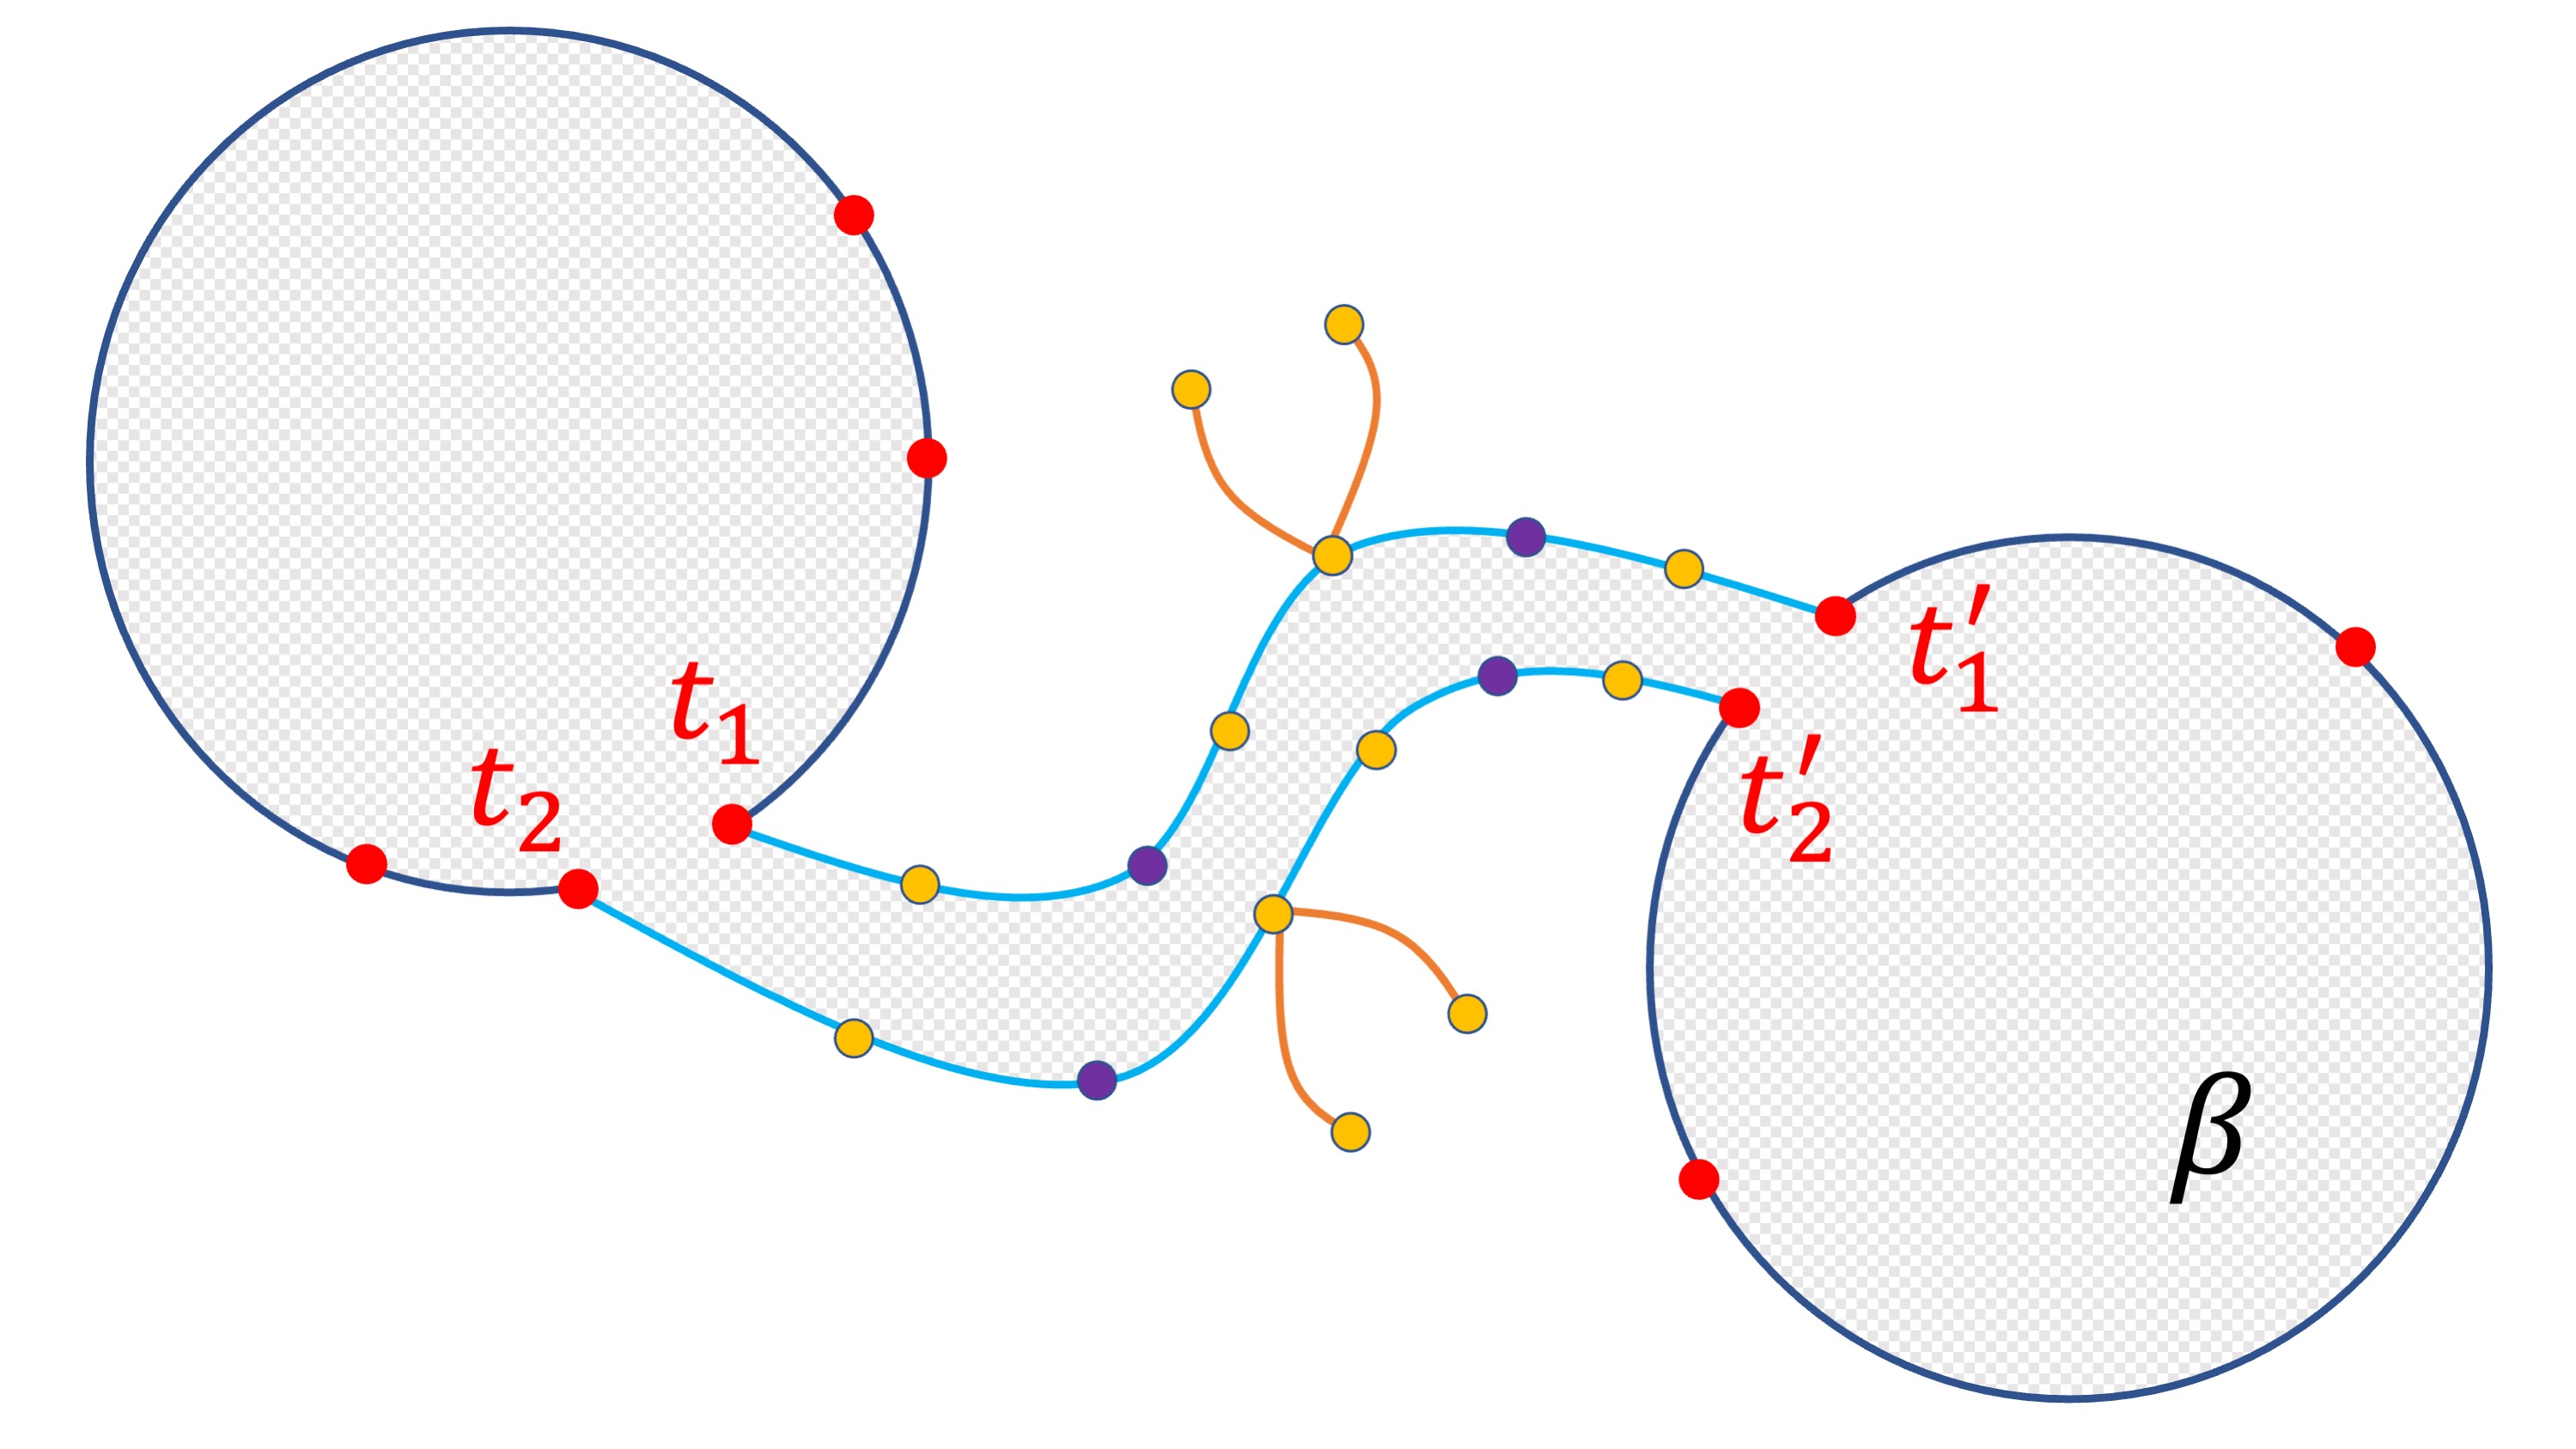
\includegraphics[scale=0.15]{fig/manyhole_2.jpg}\label{fig: splitting h-hole after}}}
	\subfigure[Graph $H$: holes $\alpha,\alpha'$ and portals are restored.]{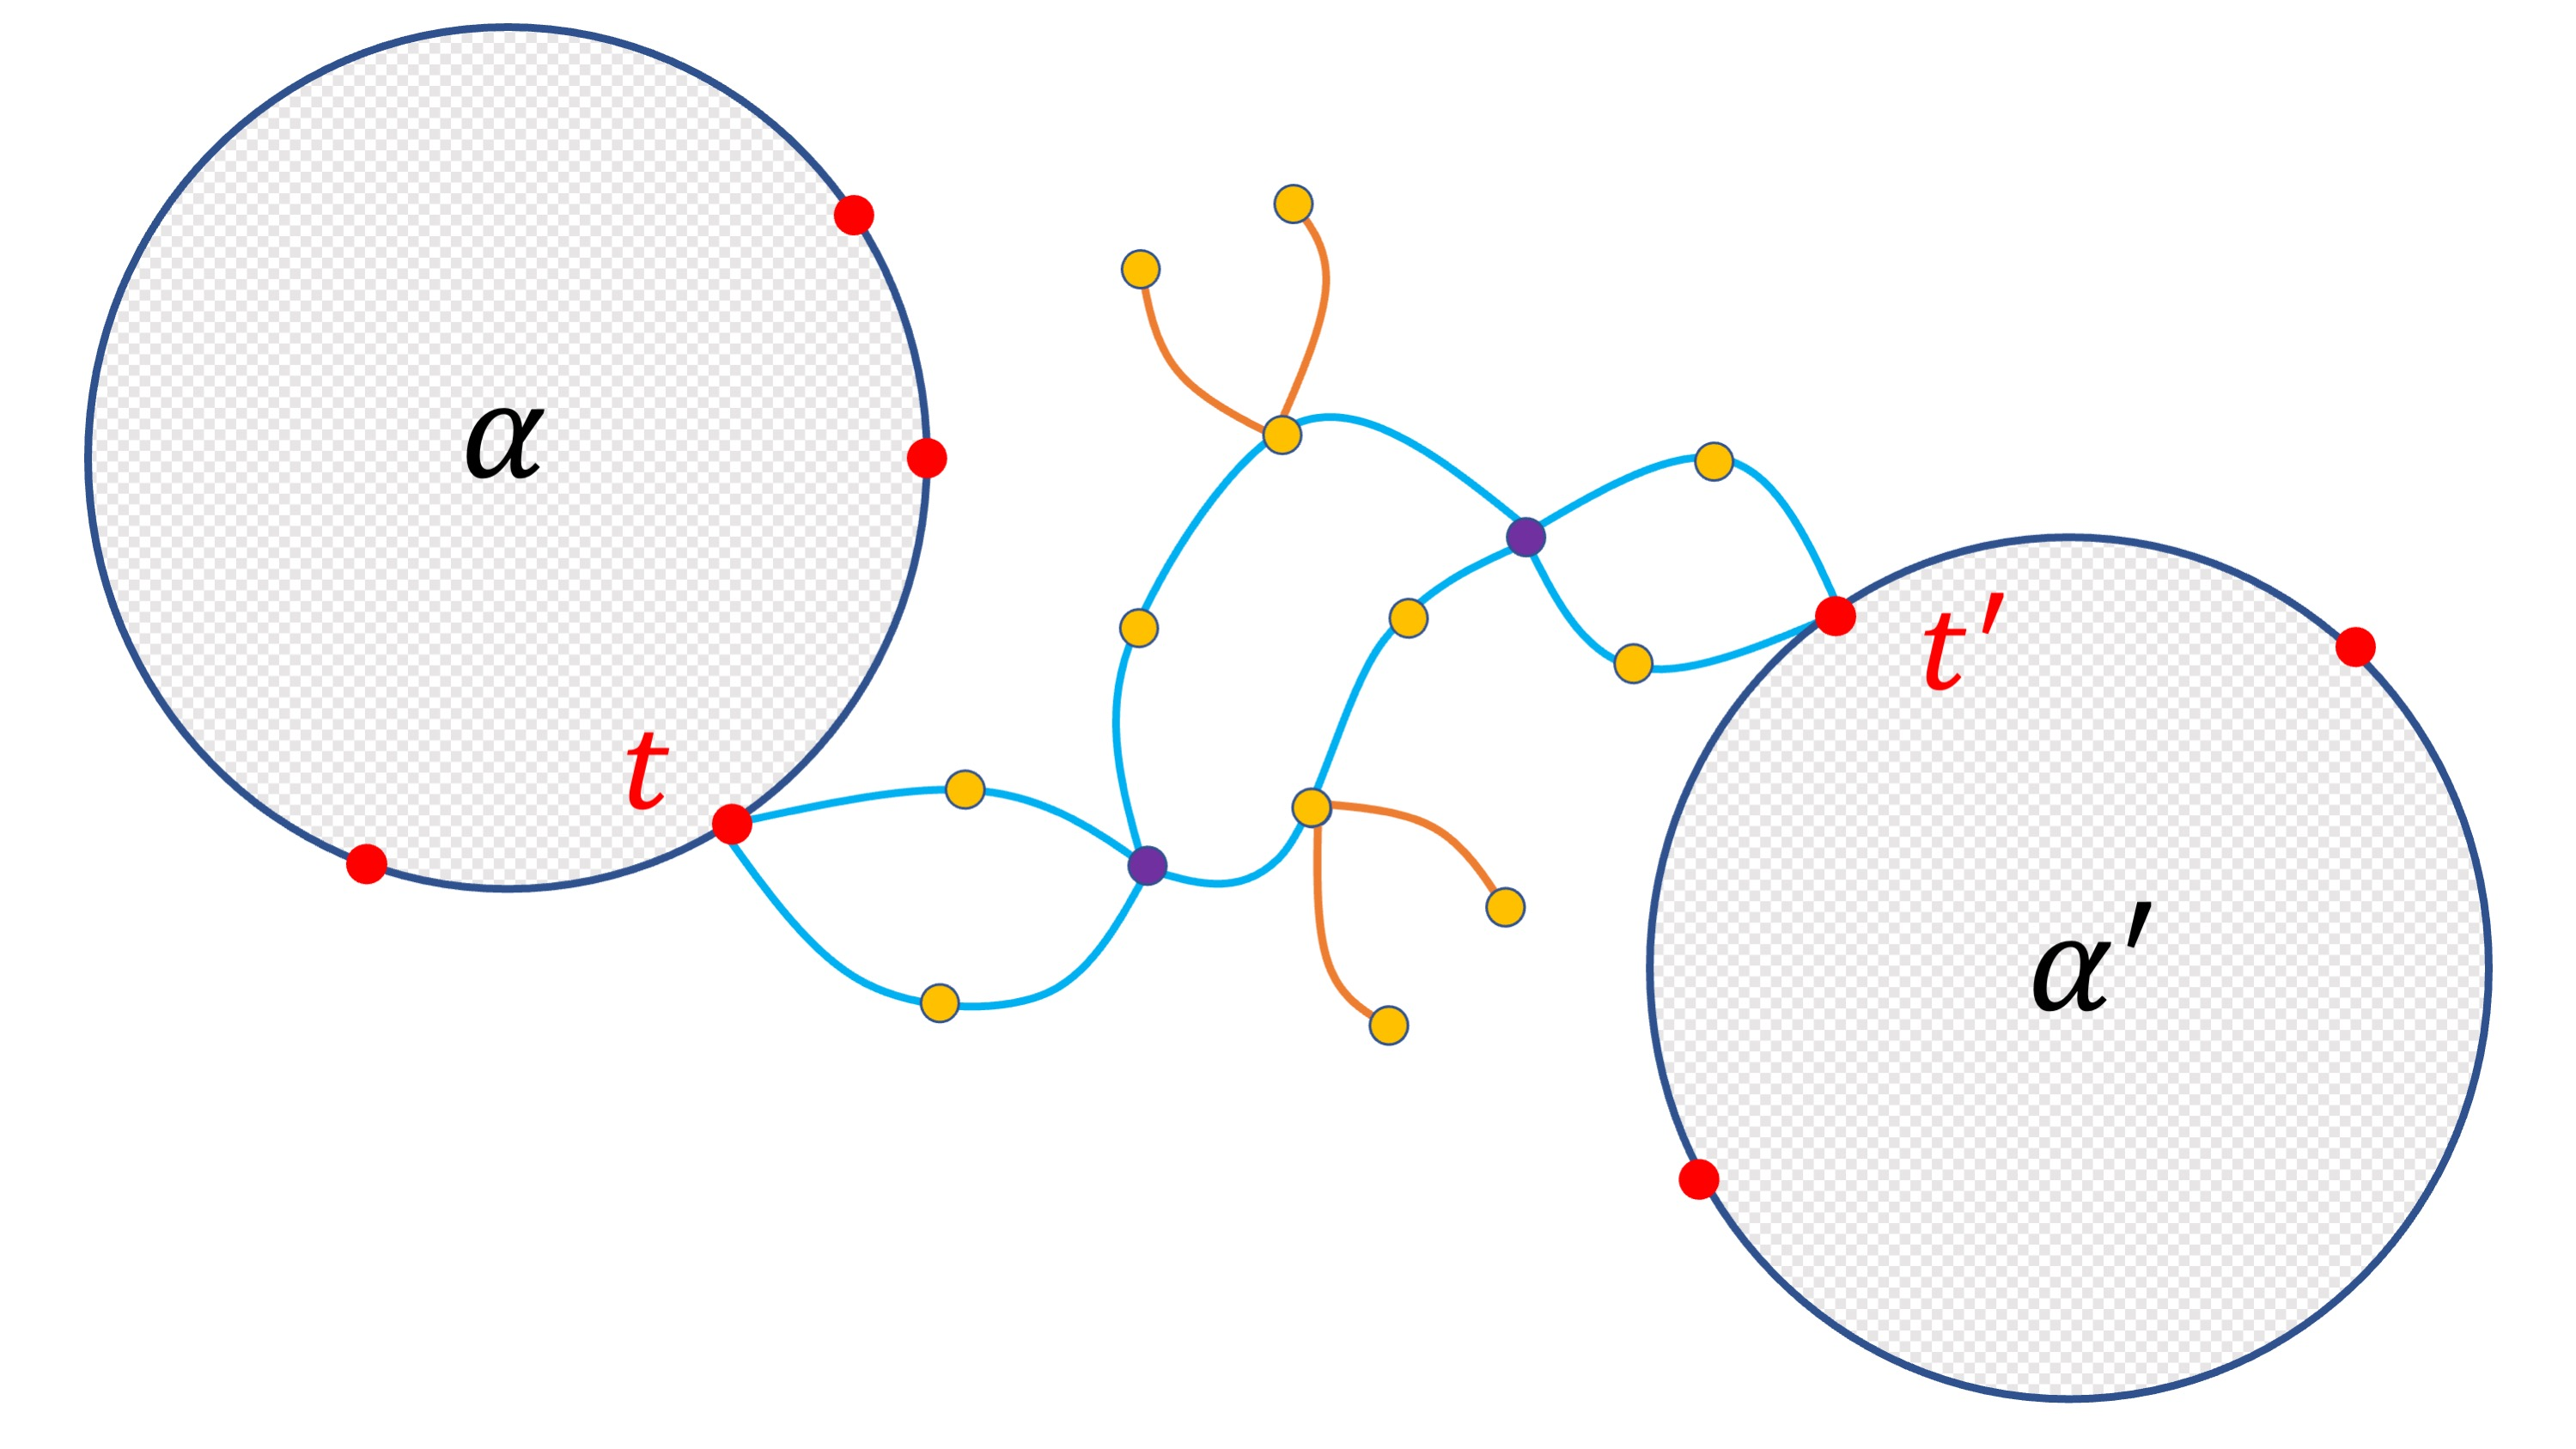
\includegraphics[scale=0.08]{fig/manyhole_3.jpg}\label{fig: gluepath_2}}
	\caption{An illustration of cutting open and gluing an $f$-face instance along path $\Pi$.\label{fig: splitting h-hole}}
\end{figure}




It remains to complete the proof by induction. We first bound the size of graph $H$.
 
\paragraph{Size of $H$.} Since graph $H$ is obtained from graph $H'$ by gluing the portals on paths $\Pi_1,\Pi_2$ back to their original vertices, $|V(H)|\le |V(H')|$, so it suffices to bound the number of vertices in $H'$.
Recall that $T'$ is the set that contains all portals and terminals in $G'$, then
%
\[
\begin{split}
|V(H')| &
\le |T'|\cdot \bigg(\frac{cf\cdot \log |T'|}{\eps''}\bigg)^{c(f-1)^2}
\le \frac{c\cdot 2^f\cdot |T|}{\eps/2f^2}\cdot \bigg(\frac{cf\cdot \log (c\cdot 2^f\cdot |T|/\eps')}{\eps\cdot (1-1/f^2)}\bigg)^{c(f-1)^2}\\
&  \le |T|\cdot \bigg(\frac{cf}{\eps}\bigg)^{c(f-1)^2+f}\cdot \bigg(\frac{\log (cf^2\cdot 2^f\cdot |T|/\eps)}{(1-1/f^2)}\bigg)^{c(f-1)^2}\\
& \le |T|\cdot \bigg(\frac{cf}{\eps}\bigg)^{c(f-1)^2+f}\cdot \bigg(\log |T|+ \log (cf^2\cdot 2^f/\eps)\bigg)^{c(f-1)^2}\\
& \le |T|\cdot \bigg(\frac{cf^2 \log |T|}{\eps}\bigg)^{cf^2},
\end{split}
\]
where we have used the previously set parameters $\eps'=\eps/2f^2$ and $\eps''=(1-1/f^2)\cdot \eps$, and the fact that $(1-\frac{1}{f^2})^{-c(f-1)^2}\le e^{c}< c^{c}$, as $c$ is large enough.



\paragraph{Quality of $H$.}
Recall that we sliced $G$ open along $\Pi$ to obtain $G'$, computed a $(1+\eps'')$ pattern emulator $H'$ for $G'$, and then glue $H'$ back to obtain $H$.
For the purpose of analysis, image that we have also glued $G'$ back to obtain $G''$. The analysis is complete by the following claims.



\begin{claim}
\label{clm: cut glue emulator}
$(H,T)$ is a quality-$(1+\eps'')$ pattern emulator for $(G'',T)$.
\end{claim}
\begin{proof}
Consider any pair $t,t'$ of terminals. 
Let $P$ be some pattern shortest path from $t$ to $t'$ in $G''$.
If $P$ contains some portal in $Y$, then we let $y^1,\ldots,y^r$ be the portals appearing on $P$ in this order.
Decompose $P$ into $r+1$ subpaths: $P^0$ between $t$ and $y^1$; for each $1\le i\le r-1$, $P^i$ between $y^{i}$ and $y^{i+1}$, and $P_r$ between $y^{r}$ and $t'$.
Assume that for each $1\le i\le r-1$, the path $P^i$ starts on the $a_i$-side of the glued paths and ends on the $b_i$-side of the glued paths, where $a_i,b_i\in \set{1,2}$. Define $a(t), b(t')\in \set{1,2}$ similarly for terminals $t,t'$.
As portals are considered as terminals in instance $G'$ and $H'$ is a quality-$(1+\eps)$ pattern emulator for $G'$ with respect to them, there exist in $H'$ 
\begin{itemize}
\item a path $Q^0$ connecting the copy $t_{a(t)}$ of $t$ to the copy $y^1_{b_0}$ of $y^1$ with the same pattern as $P^0$ in $G'$, such that $w(Q^0)\le (1+\eps'')\cdot w(P^0)$;
\item for each $1\le i\le r-1$, a path $Q^i$ connecting the copy $y^{i-1}_{a_{i}}$ of $y^{i-1}$ to the copy $y^{i}_{b_i}$ of $y^i$ with the same pattern as $P^i$ in $G'$, such that $w(Q^i)\le (1+\eps'')\cdot w(P^i)$;
\item a path $Q^r$ connecting the copy $y^r_{a_r}$ of $y^r$ to the copy $t'_{b(t')}$ of $t'$ with the same pattern as $P^r$ in $G'$, such that $w(Q^r)\le (1+\eps'')\cdot w(P^r)$.
\end{itemize}

For each $1\le i\le r-1$, as the region surrounded by $P^i$ and $P$ contains no other face, and $Q^i$ is in the same pattern with $P^i$, the region surrounded by $Q^i$ and $P$ contains no other face. Therefore, if we concatenate all these paths $Q_0,\ldots,Q_r$ in $H$, we obtain a path $Q$ connecting $t$ to $t'$ in $H$ with the same pattern as $G''$. Moreover,
\[w(Q)=\sum_{0\le i\le r}w(Q^i)\le \sum_{0\le i\le r}(1+\eps'')\cdot w(P^i)=(1+\eps'')\cdot w(P).\]
The arguments for showing that for any pattern-shortest path $Q$ from $t$ to $t'$ in $H''$, there exists a path $P$ in $G''$ with $w(P)\le w(Q)$ that has the same pattern with $Q$ is symmetric. Altogether, the proof is complete.
\end{proof}

\begin{claim}
	\label{clm: cut glue}
	$(G'',T)$ is a quality-$(1+\eps')$ pattern emulator for $(G,T)$.
\end{claim}
\begin{proof}
Consider any pair $t,t'$ of terminals. 
Let $P$ be some pattern shortest path from $t$ to $t'$ in $G$. If path $P$ is vertex-disjoint from $\Pi$, then the same path exists in $G''$, and it is easy to verify that it has the same pattern as $P$ in $G$. We assume from now on that $P$ intersects $\Pi$, and assume without loss of generality that $P$ intersects $\Pi$ at a vertex $x$ and leaves from the $1$-side.
Let $\Phi$ be the pattern of the subpath of $P$ between $t$ and $x$.
	
From the property of pattern-respecting $\eps'$-cover, there exists a vertex $y\in Y$, such that 
$$\dist^{\Phi}(t,x)\le \dist^{\Phi}(t,y)+\dist(y,x)\le (1+\eps')\cdot \dist^{\Phi}(t,x).$$ 
Consider the path in $G''$ formed by the concatenation of (i) the $\Phi$-pattern shortest path connecting $t$ to $y$; (ii) the subpath of $P_2$ connecting $y$ to $x_1$; and (iii) the copy of the subpath of $P$ between $x_1$ and $t'$.
From the inequality above, such a path has total length at most $(1+\eps')\cdot w(P)$ and has the same pattern with $P$.

On the other hand, it is easy to observe that between every pair of terminals, any pattern shortest path only has greater length in $G''$. Altogether, the proof is complete.	
\end{proof}



From \Cref{clm: cut glue} and \Cref{clm: cut glue emulator}, $(H,T)$ is a $(1+\eps'')\cdot (1+\eps')\le (1+\eps)$ pattern emulator for $(G,T)$. This completes the proof by induction of \Cref{lem: O(1) face emulator}.




\subsection{Completing the proof of \Cref{main: upper}}

In this section, we complete the proof of \Cref{main: upper} using the results in previous subsections.

\paragraph{Structured $r$-divisions.} Let $G$ be a planar graph on $n$ vertices and let $T$ be its terminals. For any integer $r>1$, a \emph{structured $r$-division} of $G$ is a collection $\gset$ of subgraphs of $G$, such that
\begin{itemize}
\item $|\gset|=O(n/r)$;
\item the edge sets $\set{E(G')\mid G'\in \gset}$ partitions $E(G)$;
\item for each $G'\in \gset$, $|V(G')|\le r$, $|T\cap V(G')|=O(1+|T|\cdot r/n)$, and if we call vertices in $G'$ that appear in some other graph in $\gset$ its \emph{boundary vertices}, then
\begin{itemize}
\item the number of boundary vertices is $O(\sqrt{r})$;
\item in the planar drawing of $G'$ induced by the planar drawing of $G$, all boundary vertices lie on $O(1)$ faces.
\end{itemize}
\end{itemize}

We use the following lemma in \cite{chang2022near} for computing structured $r$-divisions.

\begin{lemma}[Lemma 5.5 in \cite{chang2022near}]
\label{lem: r-division}
Given any planar instance $(G,T)$ and any integer $r\ge 0$, we can efficiently compute a structured $r$-division.
\end{lemma}

We now prove \Cref{main: upper}. The algorithm is simply: compute a structured $r$-division $\gset$ of the input graph $G$, construct cut sparsifiers for graphs $G'\in \gset$ using \Cref{lem: O(1) face}, and then glue them together to obtain a cut sparsifier for $G$.
It turns out that we need to apply the algorithm several times in order to obtain a near-linear size cut sparsifier, each time with different parameters $r,\eps$.

\begin{lemma}
\label{lem: recursive}
Given any planar instance $(H,U)$ and any $0<\eps<1$, we can efficiently compute a quality-$(1+\eps)$ planar cut sparsifier $(\hat H, U)$ with size $|V(\hat H)|\le O\big(\sqrt{|V(H)| |U|}\cdot (\log |V(H)|/\eps)^{c'}\big)$, for some universal constant $c'>0$.
\end{lemma}

\begin{proof}
Denote $n=|V(H)|$ and $k=|U|$. Let $c'$ be a constant greater than the square of the product of the constant $c$ in \Cref{lem: O(1) face} and all hidden constants in the definition of structured $r$-divisions.

We first compute a structured $r$-division for $H$ with $r=n/k$ using the algorithm from \Cref{lem: r-division}, and obtain a collection $\hset$ of subgraphs of $H$, each being a $O(1)$-face instance. We then apply the algorithm from \Cref{lem: O(1) face} to each $H'\in \hset$ and obtain a $(1+\eps)$-cut sparsifier $\hat H'$, and finally glue all of them together to obtain $\hat H$.
From \Cref{lem: O(1) face} (here note that $f=O(1)$ and $f^2c\le c'$),
\[
|V(\hat H)|\le \sum_{H'\in \hset}|V(\hat H')|\le O\bigg(k\cdot \sqrt\frac{n}{k}\bigg)\cdot \bigg(\frac{cf \log n}{\eps}\bigg)^{cf^2}\le O\bigg(\sqrt{nk}\cdot \bigg(\frac{\log n}{\eps}\bigg)^{c'}\bigg).
\]
From \Cref{lem: divide}, the graph $\hat H$ is a quality-$(1+\eps)$ planar cut sparsifier. 
%It is also easy to verify that the construction in the proof of \Cref{lem: divide} preserves planarity.
 This completes the proof.
\end{proof}


We now complete the proof of \Cref{main: upper} using \Cref{lem: recursive}. We start by applying the algorithm in \cite{krauthgamer2017refined} to obtain an exact cut sparsifier $(G_0,T)$ of $(G,T)$ with $|V(G)|=2^{2k}\cdot \poly(k)\le 2^{3k}$.
Then the algorithm consists of two phases.

In the first phase, we set parameters $L=\log k$ and $\eps'=\eps/6L$, and sequentially for each $i=1,\ldots,L$, we apply algorithm \Cref{lem: recursive} to graph $G_{i-1}$ to obtain graph $G_i$.
We show that $|V(G_L)|=(k/\eps)^{O(1)}$ (applying the next lemma with $i=L=\log k$).

\begin{claim}
For each $1\le i\le L$, $|V(G_i)|\le 2^{3k/2^i}\cdot (18k\log k/\eps)^{4c'}$.
\end{claim}
\begin{proof}
We prove by induction on $i$. The claim is true for $i=0$.
From \Cref{lem: recursive},
\[
\begin{split}
|V(G_i)| & \le \sqrt{|V(G_{i-1})|\cdot k}\cdot \bigg(\frac{\log (2^{3k})}{\eps'}\bigg)^{c'}
\le 
\sqrt{|V(G_{i-1})|}\cdot k\cdot\bigg(\frac{3k}{\eps/6\log k}\bigg)^{c'}\\
& \le \sqrt{2^{3k/2^i}\cdot (18\log k/\eps)^{4c'}}\cdot\bigg(\frac{3k}{\eps/6\log k}\bigg)^{2c'}\\
& \le 2^{3k/2^{i+1}}\cdot (18\log k/\eps)^{2c'}\cdot \bigg(\frac{3k}{\eps/6\log k}\bigg)^{2c'}
\le 2^{3k/2^i}\cdot (18k\log k/\eps)^{4c'}.
\end{split}
\]
\end{proof}

In the second phase, we set parameters $\bar L=2\log k\log k$ and $\bar\eps'=\eps/6L$, and sequentially for each $i=1,\ldots,\bar L$, we apply algorithm \Cref{lem: recursive} to graph $G_{L+i-1}$ to obtain graph $G_{L+i}$.

\begin{claim}
	For each $1\le i\le \bar L$, $|V(G_{L+i})|\le k^{1+5c'/2^i}\cdot (5c'\log k/\bar\eps')^{2c'}$.
\end{claim}
\begin{proof}
	We prove by induction on $i$. The claim is true for $i=0$.
	From \Cref{lem: recursive},
	\[
	\begin{split}
	|V(G_{L+i})| & \le \sqrt{|V(G_{L+i-1})|\cdot k}\cdot \bigg(\frac{\log (k^{5c'})}{\bar\eps'}\bigg)^{c'}
	\le 
	\sqrt{|V(G_{L+i-1})|}\cdot \sqrt{k}\cdot\bigg(\frac{5c'\log k}{\bar\eps'}\bigg)^{c'}\\
	& \le  k^{\frac{1}{2}\cdot (1+1+5c'/2^{i-1})}\cdot \sqrt{(5c'\log k/\bar\eps')^{2c'}}\cdot\bigg(\frac{5c'\log k}{\bar\eps'}\bigg)^{c'}\\
	& \le k^{1+5c'/2^i}\cdot (5c'\log k/\bar\eps')^{2c'}.
	\end{split}
	\]
\end{proof}
Applying $i=\bar L$, we get that $|V(G_{L+\bar L})|\le O(k\cdot \poly(\log k/\eps))$ (as $c'$ is a universal constant).

On the other hand, from \Cref{obs: chain}, we get that instance $(G_{L+\bar L},T)$ is a cut sparsifier of  instance $(G,T)$ with quality
$(1+\eps/6L)^L\cdot (1+\eps/6\bar L)^{\bar L}\le (1+\eps)$. The proof is complete.









